\documentclass{article}
\usepackage[margin=1in]{geometry}
\usepackage{booktabs,graphicx,xcolor,hyperref}
\hypersetup{colorlinks=true,linkcolor=blue,urlcolor=blue}
\title{Love AI More. Trust AI Less.\\A Data-to-LaTeX Reasoning Walkthrough}
\author{Discrete Structures and Critical Thinking}
\date{}
\begin{document}\sloppy\maketitle
\begin{abstract}AI can help us generate explanations, code, and hypotheses. It cannot remove our obligation to check what a measurement means. This short report models a reusable workflow on concurrency data from a local-model benchmark.\end{abstract}

\section{Opening hook: a plausible answer can still be wrong}
Ask the class: \emph{“If we send more requests to an AI server and the total tokens per second rises, did the GPU become faster?”} An AI answer might confidently say yes. Today we test that answer. The lesson is not anti-AI: use it to suggest hypotheses, then make the evidence earn trust.

\section{Claim and why it matters}
\textbf{Claim.} Increasing the number of simultaneous requests should increase aggregate throughput until the available parallelism is saturated. The tempting shortcut “bigger GPU = faster” is not precise enough: it mixes hardware, scheduling, setup overhead, and memory placement.

\section{Evidence: a reproducible table}
The source is a clean derivation of 24 benchmark observations: four hardware/parallel-setting series, each tested at six batch sizes. Each cell is aggregate tokens/second followed by the overlap factor, computed as aggregate rate divided by median per-request generation rate.
\begin{center}\begin{tabular}{llrrrr}\toprule
Hardware & parallel limit & $N=1$ & $N=4$ & $N=8$ & $N=32$\\\midrule
Tesla T4 & 1 & 69.2 / 0.49 & 74.1 / 0.54 & 73.4 / 0.53 & 73.4 / 0.54\\
Tesla T4 & 8 & 72.6 / 0.53 & 102.8 / 2.18 & 117.3 / 4.77 & 121.9 / 4.84\\
GTX 1060 3 GB & 1 & 59.6 / 0.61 & 84.5 / 0.86 & 90.2 / 0.92 & 94.6 / 0.98\\
GTX 1060 3 GB & 4 & 73.6 / 0.99 & 112.1 / 3.76 & 120.7 / 3.98 & 119.9 / 3.97\\
\bottomrule
\multicolumn{6}{l}{\scriptsize Each cell: aggregate tokens/s \,/\, overlap factor.}\\
\end{tabular}
\end{center}

\section{Evidence: see the shape}
\begin{figure}[h]\centering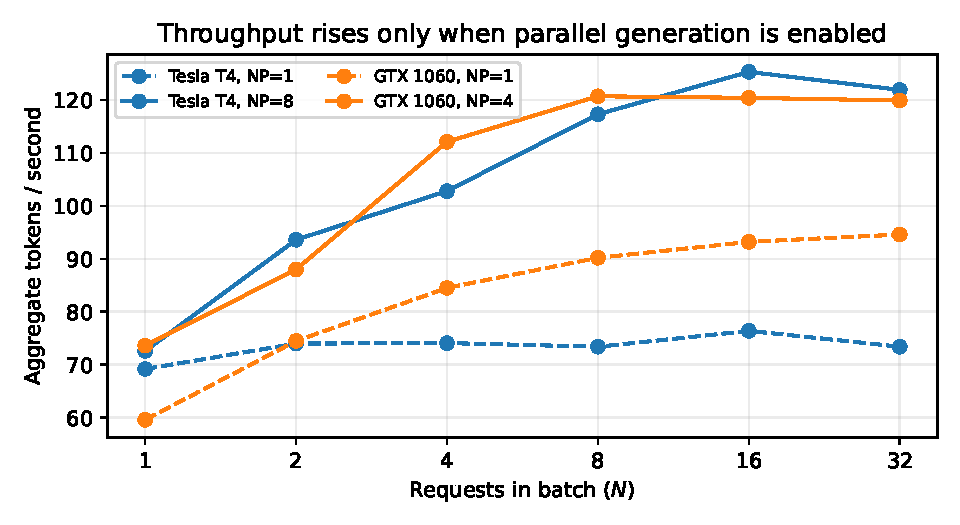
\includegraphics[width=.92\linewidth]{../generated/figures/throughput.pdf}\caption{More requests help when genuine parallel generation is available. Dashed lines have parallel limit 1; solid lines have limits 8 or 4.}\end{figure}

\section{Reading the result}
With parallel limit 1, throughput approaches one stream: the GTX 1060 rises from 59.6 to 94.6 tokens/s as setup overhead is hidden, but it never demonstrates four requests generating at once. With limit 8, the T4 reaches 125.3 tokens/s at $N=16$ and then levels off. With limit 4, the GTX 1060 reaches 120.7 at $N=8$ and then levels off. Thus the knee is near the parallel limit, not automatically at the largest batch size.

\section{Discrete structures connection: relations and counting}
Order the observations by $N\in\{1,2,4,8,16,32\}$ and define a relation $N_i\preceq N_j$ when $N_i\leq N_j$. The claim predicts a nondecreasing throughput relation, but the T4 limit-8 series falls from 125.3 at 16 to 121.9 at 32: the relation is not strictly monotone. The experiment's design is also a product-rule count: 4 series $\times$ 6 batch sizes $=24$ observations. Conditioning on a parallel limit is the logical move that prevents comparing unlike cases.

\section{Assumptions, caveats, and the check}
\begin{itemize}
\item Token counts and per-request rates are roughly comparable across a series.
\item The parallel limit is derived from the experiment setting; the probe recorded the server value as ``auto'' in some runs.
\item GPU placement is an outcome: the 3 GB card's limit-4 run was 84\% GPU / 16\% CPU.
\item Placement and ambient load can confound a cross-machine comparison; direct generation timing would improve the study.
\end{itemize}
The check is the overlap ratio. At T4 limit 8 and $N=16$, $125.3/25.5\approx4.91$, so about five requests were genuinely generating at once. At T4 limit 1 and $N=16$, $76.4/138.3\approx0.55$, so the rising curve is overhead being hidden, not batching.

\section{Confidence decision}
\fcolorbox{black}{yellow!20}{\parbox{.92\linewidth}{\textbf{Decision: medium-high confidence, bounded claim.} More concurrency helps until the configured parallelism saturates in these measured settings. “Bigger GPU = faster” is not a safe universal conclusion.}}

\section{Instructor notes and student worksheet}
\textit{Suggested prompt:} “Point to the claim, evidence, assumptions, check, and confidence sentence. Which one would an AI-generated answer most likely blur?” Emphasize that the overlap calculation is a proof-like check: it tests whether the data measures the proposed mechanism.

\paragraph{Activity (5 minutes).} In pairs, choose one series. Write (1) a one-sentence claim, (2) two numbers as evidence, (3) one assumption, and (4) an overlap-ratio check. Mark the claim supported, refuted, or undecidable. Share one disagreement.

\paragraph{Reflection.} What would you measure next to distinguish “the GPU is saturated” from “setup overhead is hidden”? Why would that measurement change your confidence?

\paragraph{15-minute flow.} 0--2 hook and prediction; 2--4 claim/evidence workflow; 4--7 table and relation/counting connection; 7--10 plot and knee; 10--12 overlap check; 12--15 pairs activity and reflection.
\end{document}
